\documentclass{article}
% Teacher-supplied style is copied byte-for-byte; preprint shows the named authors.
\usepackage[preprint,nonatbib]{neurips_2021}
\usepackage[utf8]{inputenc}
\usepackage[T1]{fontenc}
\usepackage{hyperref,url,booktabs,amsfonts,microtype,xcolor,graphicx,tabularx,array,capt-of}
\hypersetup{hidelinks,pdftitle={Credit Card Default Prediction},pdfauthor={SC6122 Group 5}}
% Course metadata only: do not imply submission to or acceptance by NeurIPS.
\makeatletter
\renewcommand{\@noticestring}{NTU SC6122 Emerging Topics in FinTech --- Group 5 course project.}
\makeatother
\title{Credit Card Default Prediction:\\Ranking Risk and Choosing an Action}
\author{ {{MEMBER_AUTHORS}} }
\begin{document}
\maketitle
\thispagestyle{plain}
\begin{abstract}
We compare logistic regression, a decision tree, random forest and XGBoost on 30,000 historical credit-card clients. Shared fitting, validation and test partitions separate hyperparameter selection from threshold choice. Tree regularization improves the decision-tree baseline; selected RF and XGBoost have similar test average precision. XGBoost tuning does not improve test ranking, but a validation-selected threshold reduces hypothetical cost by {{XGB_REDUCTION}}\% under a 5:1 missed-default-to-false-alarm cost ratio. The policy flags 55.72\% of clients, exposing a substantial review burden. The results distinguish predictive ranking from action policy and support further validation with realistic costs and capacity limits, rather than immediate deployment.
\end{abstract}
\section{Problem, objectives and data}
Credit default prediction can support the prioritization of account reviews. A missed default and an unnecessary review impose different costs, so the model with the best classification accuracy need not support the best decision. We ask: \textbf{how well can models identify default risk, and how should ranking ability, interpretability and decision cost be balanced?} We compare logistic regression (LR), a decision tree (DT), random forest (RF) and XGBoost on the same historical records. Objectives are to evaluate ranking using average precision (AP) and ROC-AUC, explain predictive associations, and examine threshold policies under explicit hypothetical error costs.

We use UCI's Default of Credit Card Clients dataset \cite{uci}: 30,000 Taiwan clients, 23 predictors and a binary default-payment outcome (1 = default). Predictors describe credit limit, age, sex, education, marital status, repayment status, bill amounts and previous payments. Payment history covers April--September 2005; monetary variables are in NT dollars. There are 6,636 positive outcomes (22.12\%) and 23,364 negatives. Thus an always-negative classifier can look accurate while detecting no defaults. This is an educational historical-sample study, not evidence of readiness for current credit decisions.

\textbf{Cleaning and identity.} There are no missing entries. Undocumented EDUCATION values 0/5/6 are mapped to 4 (345 rows); MARRIAGE 0 is mapped to 3 (54 rows). Other values, including negative repayment codes and large or negative amounts, are retained. No rows, outliers or duplicate records are removed; 35 identical feature--label repetitions remain. Equal records alone do not establish repeated customers, but retaining them can create dependence across partitions. The final audit finds {{DUP_TEST}} test rows whose feature vectors also appear in development data. This limitation is retained rather than changing the established split after evaluation.

\textbf{Traceability.} The official UCI CSV was downloaded again during integration, and the above transformation reproduces the committed clean file exactly in values, types, row order and column order. The original download bytes were not saved; the new raw file and SHA256 audit are provided. The repository's zero-based \texttt{row\_id} equals original UCI ID minus one. Neither identifier nor the label enters any model.
\begin{center}
\begin{minipage}{\linewidth}
\captionof{table}{Fixed stratified partitions (seed 42). Inner CV uses 14,400 fitting and 3,600 holdout rows per fold.}
\label{tab:split}\centering
\begin{tabularx}{\linewidth}{@{}lrX@{}}\toprule
Partition & Clients & Purpose\\\midrule
Fitting & 18,000 & Five-fold CV; final fitting with selected parameters\\
Validation & 6,000 & Selection of decision thresholds\\
Test & 6,000 & Evaluation of frozen models and decisions\\\bottomrule
\end{tabularx}
\end{minipage}
\end{center}
\section{Experimental design and model selection}
The original 80/20 split yields 24,000 development and 6,000 test rows. A further stratified 75/25 development split produces 18,000 fit and 6,000 validation rows. Positive counts are {{FIT_POS}}, 1,327 and 1,327 respectively. All four reproducible experiments have identical row-level development and five-fold CV memberships. IDs are unique and partitions disjoint. Final models fit only the 18,000 rows; validation rows are not incorporated by a later refit.

Each CV training fold fits its own preprocessing. SEX, EDUCATION and MARRIAGE are one-hot encoded with unknown categories ignored. LR additionally learns numeric StandardScaler statistics within the fold. Tree models retain numeric scales. No missing-value imputation or sampling is used. Selected class weights are part of the training configuration, not a change to test prevalence. Pipelines prevent categories or scaling moments from being learned on validation/test data.

\textbf{Hyperparameters.} The common selection objective is mean five-fold AP. Equal scores prefer the lowest candidate index. DT uses exhaustive grid search; RF/XGBoost evaluate a specified baseline plus 23 seeded random candidates. The harmonized LR run evaluates 12 exhaustive settings. These are comparable splits and objectives, not identical computational budgets.
\begin{center}
\begin{minipage}{\linewidth}
\captionof{table}{Declared search budgets and selected configurations. Complete settings and per-fold scores accompany the frozen protocols.}
\centering
{{CONFIG_TABLE}}
\end{minipage}
\end{center}

LR uses L2 logistic regression (\texttt{lbfgs}, maximum 3,000 iterations); its grid crosses $C$ values .001, .01, .1, 1, 10 and 100 with no class weighting or balanced weighting. DT searches maximum depth 2, 3, 4, 5, 6, 8 or unlimited, and minimum leaf size 1, 20 or 100. RF varies tree count, depth, split/leaf size, feature subsampling and class weighting. XGBoost varies tree count, learning rate, depth, child weight, row/column sampling, L1/L2 penalties and positive-class weighting \cite{xgboost}. Baseline tree/ensemble configurations are retained alongside selected configurations.

\textbf{Decision selection.} We use $\hat y=1[s\geq t]$ throughout, where $s$ is the positive-class score. The fixed reference is $t=0.5$. For LR, RF and XGBoost, all distinct validation score cutoffs are considered for $C_r=FP+r\,FN$, with $r\in\{1,3,5,10\}$. Equal costs prefer the largest threshold (fewer alerts); tied scores move together. DT has only its historical fixed 0.5 policy. Each cost threshold is chosen on validation, then applied unchanged to test predictions. No test threshold sweep is used to select a policy.

\textbf{LR contribution and comparison scope.} Lei Peng contributed data inspection, preprocessing and the initial LR baseline; the team's earlier LR result tables are retained in the repository. For the common comparison below, LR* denotes a separately logged integration run using the shared fitting rows, CV folds and metric implementation. Its 12-setting search was specified before that run, and its model and thresholds were frozen before test evaluation. This was a \emph{post-hoc harmonization after earlier test results were available}, not a fresh independent holdout. The reported LR* values refer to that run, not a claim to reproduce the teammate's original execution. All models retain the limitation of team-wide historical test exposure.
\section{Ranking and classification findings}
\begin{center}
\begin{minipage}{\linewidth}
\captionof{table}{Test performance at threshold 0.5 ($n=6,000$; default positive). P/R/F1/Acc are proportions; B = baseline, T = CV-selected. LR* is the integration run described in Section 2.}
\centering
{{PERFORMANCE_TABLE}}
\end{minipage}
\end{center}

\begin{center}
\begin{minipage}{\linewidth}
\captionof{table}{Test confusion counts at 0.5, recomputed from row-aligned scores and labels. B = baseline; T = CV-selected.}
\centering
{{CONFUSION_TABLE}}
\end{minipage}
\end{center}

AP is computed by \texttt{average\_precision\_score}, a recall-increment weighted sum of precision, not trapezoidal PR-AUC \cite{ap}. ROC-AUC summarizes positive--negative score ordering. Both use continuous scores and are independent of the chosen operating threshold; precision, recall, F1 and accuracy describe a particular decision rule.
\begin{center}
\begin{minipage}{\linewidth}
\centering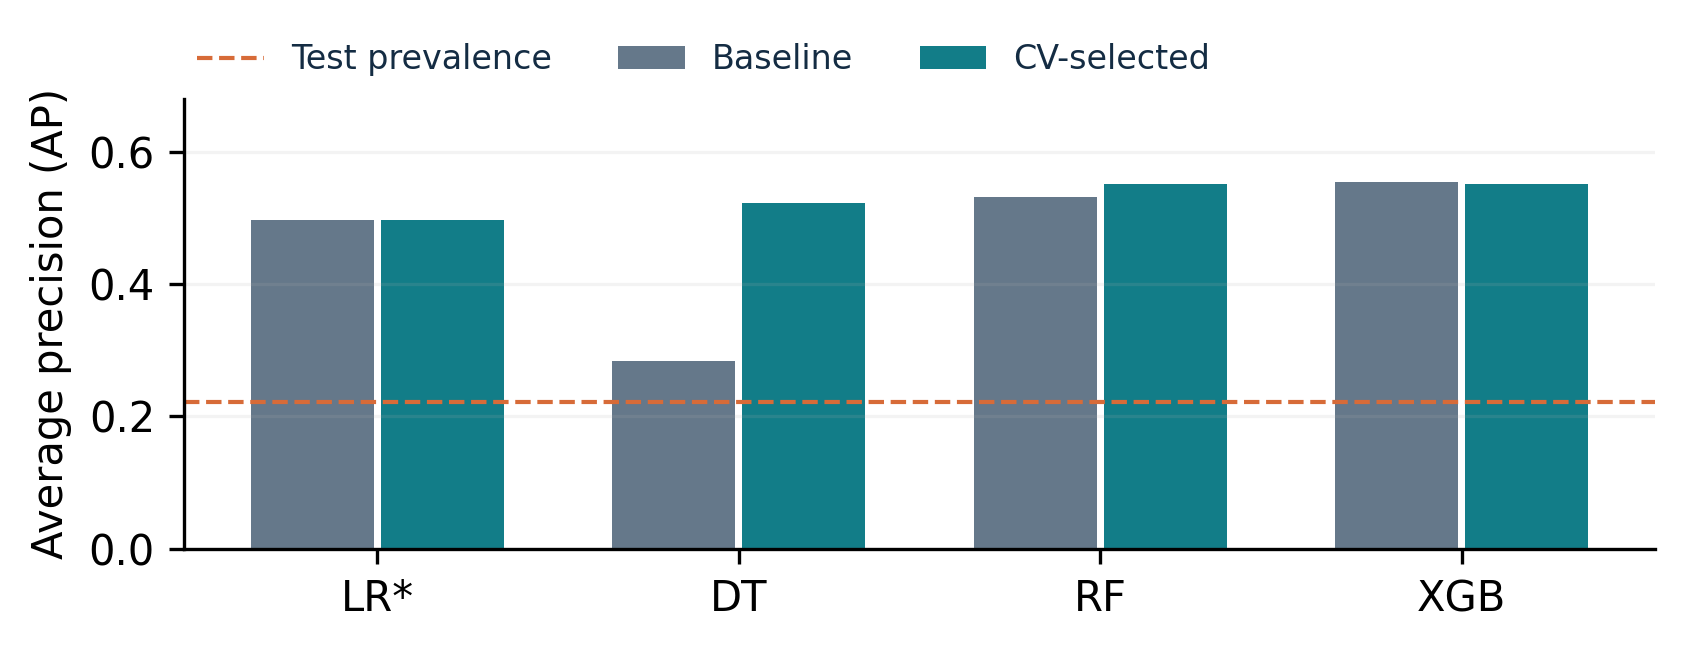
\includegraphics[width=\linewidth]{figures/ranking.png}
\captionof{figure}{Test AP for declared baselines and CV-selected models. The dashed reference is positive prevalence (0.2212). Selection uses fit-fold CV, never this chart.}
\end{minipage}
\end{center}

The unrestricted DT strongly overfits: mean fit-fold AP is about 1.0000 while CV AP is 0.2970. A minimum leaf size of 100 raises test AP from 0.2843 to 0.5221. RF selection raises AP from 0.5312 to 0.5508. XGBoost changes from 0.5544 to 0.5516: the selected configuration does not improve test ranking. LR* changes from {{LR_BASE_AP}} to {{LR_TUNE_AP}}, also without a ranking gain. Among the displayed point estimates the XGBoost baseline has the highest AP, but this retrospective observation does not authorize a new model-selection round. Small differences between RF and XGBoost do not establish superiority.
\section{Thresholds, costs and review capacity}
We treat one false-positive review as one hypothetical cost unit, and a missed default as $r$ units. This is a sensitivity analysis, not a measured monetary loss: loan exposure, loss given default, treatment effects and review capacity are unavailable. Positive class weights can change score calibration, so a probability-derived cutoff such as $1/(1+r)$ is not assumed valid. Policies are selected empirically on validation data.
\begin{center}
\begin{minipage}{\linewidth}
\captionof{table}{Same-model test comparison at 0.5 and the validation-selected $r=5$ policy. Alerts and recall are percentages; cost is FP + 5 FN across 6,000 clients. DT has no historical validation-selected cost policy.}
\centering
{{COST_TABLE}}
\end{minipage}
\end{center}
\begin{center}
\begin{minipage}{\linewidth}
\centering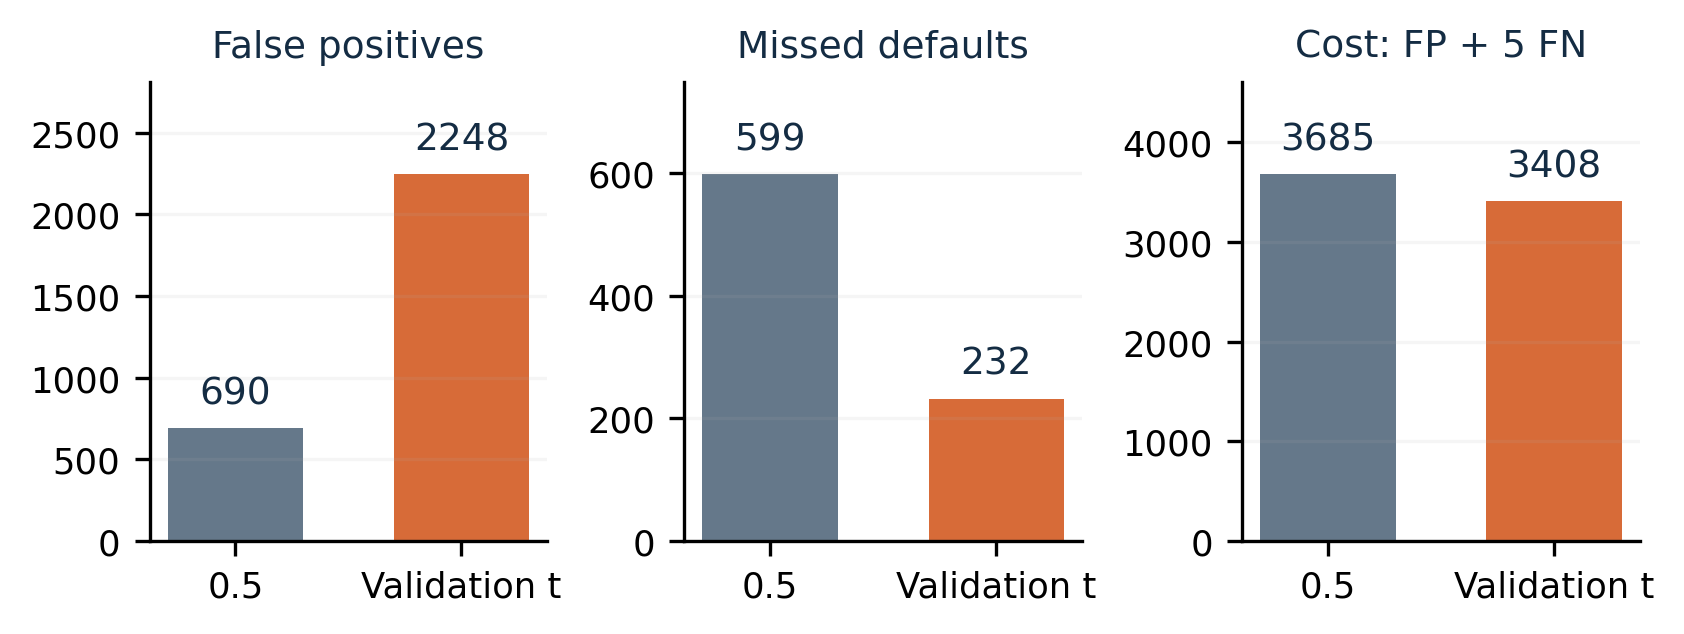
\includegraphics[width=\linewidth]{figures/cost_tradeoff.png}
\captionof{figure}{Moving the same tuned XGBoost from 0.5 to its validation cutoff changes FP/FN and workload. Ranking scores remain unchanged.}
\end{minipage}
\end{center}

For XGBoost, $t={{XGB_THR}}$ changes cost from 3,685 to 3,408, a reduction of {{XGB_REDUCTION}}\%. Recall rises from 54.86\% to 82.52\%, while false positives rise from 690 to 2,248 and 55.72\% of clients are flagged. Precision falls from 51.34\% to 32.76\%. The benefit is fewer missed defaults under the assumed cost ratio; it is not a gain in AP or ROC-AUC. If that review load is infeasible, the policy would need a separately validated capacity constraint, not a threshold changed after viewing test errors.

RF at its validation $r=5$ threshold costs 3,404 and flags 48.45\%, versus XGBoost's 3,408 and 55.72\%. The four-unit difference is too small to support a strong cross-model cost claim. RF detects fewer defaults (77.09\% recall) with fewer false positives. An always-negative policy costs 6,635 and an always-positive policy 4,673 at $r=5$; both are useful context, not deployment recommendations.

\textbf{Uncertainty.} Historical 1,000-replicate stratified paired bootstraps condition on the frozen models, thresholds and fixed class counts. XGBoost's tuned-minus-baseline AP difference is $-0.0028$ (95\% interval $[-0.0106,0.0054]$). The selected-minus-0.5 cost difference is $-46.17$ units per 1,000 (95\% interval $[-74.34,-18.00]$). These intervals describe resampling of fixed predictions; they exclude retraining, hyperparameter/threshold selection, prevalence shifts and new-population uncertainty. They cannot be read as end-to-end deployment guarantees.
\section{Interpretation and audit evidence}
\textbf{Complementary explanations.} LR coefficients summarize regularized associations on standardized numeric and encoded categorical scales. Correlated bill/payment variables and full one-hot coding limit isolated coefficient interpretations. DT offers explicit paths: its root splits on \texttt{PAY\_0 <= 1.5}; within fit rows, default proportions are 16.51\% on the left and 70.13\% on the right. These are node-level sample summaries, not causal effects or calibrated individual probabilities. The selected tree has 134 leaves and depth 18: no explicit depth cap does not mean no regularization, since every leaf requires at least 100 observations.

RF averages many trees, making full decision paths less concise. Its saved validation permutation importance identifies recent repayment status, PAY\_0, as most influential: shuffling it reduces AP by {{RF_TOP_IMPORTANCE}} on average, versus {{RF_SECOND_IMPORTANCE}} for PAY\_2. Correlated variables can substitute for one another, and shuffling can create unrealistic combinations; importance describes predictive reliance, not causality. XGBoost instead builds regularized trees sequentially; its threshold trade-offs are evaluated in Section 4.
\begin{center}
\begin{minipage}{\linewidth}
\centering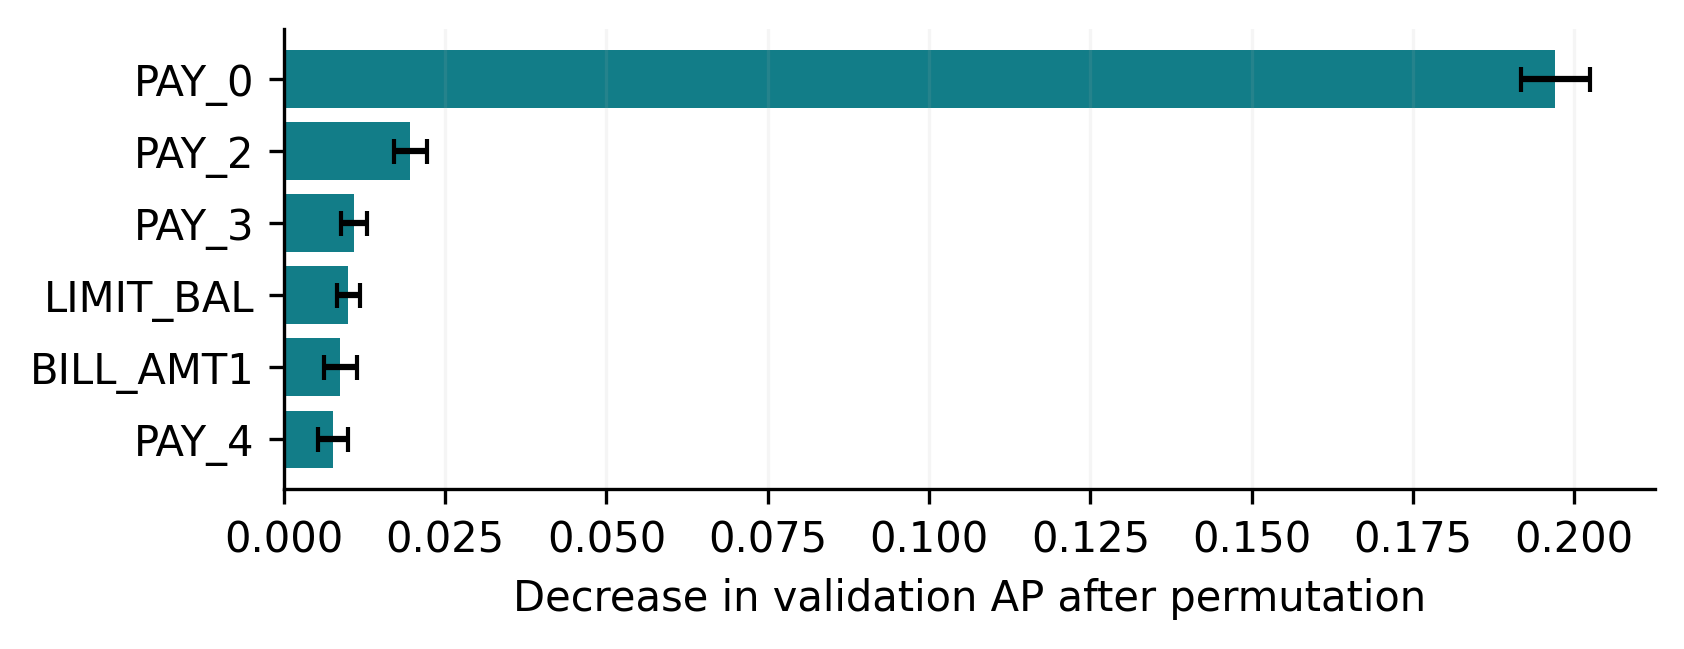
\includegraphics[width=\linewidth]{figures/importance.png}
\captionof{figure}{Tuned random-forest validation permutation importance, top six features. Error bars are the SD across five permutations, not confidence intervals or causal estimates. Horizontal units: decrease in validation AP.}
\end{minipage}
\end{center}

\textbf{Illustrative RF errors.} At 0.5, the selected forest has 637 false negatives and 573 false positives. In the existing saved error export, row {{RF_FN_ROW}} defaults despite score {{RF_FN_SCORE}} and PAY\_0={{RF_FN_PAY}}; row {{RF_FP_ROW}} does not default despite score {{RF_FP_SCORE}} and PAY\_0={{RF_FP_PAY}}. These most-confident errors illustrate that repayment history is not deterministic; they are not representative average clients and are not used to retune the model. Both threshold-specific case exports satisfy their own classification rules. Extreme cases can remain errors under both policies even when overall error counts change.

\textbf{Reconciliation.} All metrics in the final comparison are recalculated after one-to-one \texttt{row\_id} alignment with actual labels. CSV scores and thresholds use round-trip float parsing. Threshold-equality cases are explicitly tested with $\geq$; no rounding is performed before decisions. Source-train/test hash differences in historical protocols are explained by LF/CRLF serialization, while parsed content, types and order agree. Development and CV membership files are identical across the reproducible models.

Saved models reproduce stored decisions. XGBoost probability replay on this platform differs by at most $5.96\times10^{-8}$ (float32-scale drift) while frozen policy decisions agree; original probabilities remain the reporting source. Model hashes and run metadata are checked, with newline-aware evidence for textual artifacts \cite{repo}. Audit checks establish reproducible evidence consistent with the code and artifacts; they cannot prove everything a teammate did outside the repository.
\section{Conclusions, limitations and contributions}
The historical sample contains useful predictive structure. A regularized tree improves on its unrestricted baseline and provides inspectable rules. RF and XGBoost obtain similar selected-model AP, while LR supplies an interpretable linear reference under the common comparison protocol.

\textbf{Ranking quality and action policy answer different questions.} XGBoost tuning did not yield a clear AP gain, but its validation-selected cutoff reduced hypothetical cost by accepting more false positives. Operational selection needs credible error costs and review capacity; test outcomes cannot justify another optimization round.

Limitations include one historical geography/time period; a random rather than temporal or external holdout; retained duplicate feature vectors; reuse of a previously examined test sample; unequal search budgets; unvalidated calibration; and no assessment of group-specific errors or fairness. Demographic fields warrant further governance evaluation. Cost ratios do not capture exposure, realized losses, intervention benefits or review limits. The conditional bootstrap omits the uncertainty from building and selecting models. We make no causal, regulatory-compliance or production-readiness claim.

A defensible next study would freeze a new protocol on fresh temporal/external data, assess calibration and subgroup errors, collect realistic loss and intervention-cost estimates, and evaluate policies constrained by review capacity. These are future steps, not experiments silently performed on the already evaluated test set.

\section*{Member contribution statement}
\begin{center}
\begin{minipage}{\linewidth}
\captionof{table}{Member responsibilities and equal contribution shares.}
\centering
{{MEMBER_CONTRIBUTIONS}}
\end{minipage}
\end{center}
Shared responsibilities cover the data split, preprocessing and metrics, integration of the four sections, result checking and presentation preparation.

\section*{AI disclosure}
Generative AI was used for language polishing and grammar guidance, and to assist with code development, experiment verification, analysis, and preparation of the report and presentation. The group is responsible for the submitted work, its interpretation and the appropriate acknowledgement of sources.

{\small
\begin{thebibliography}{9}
\bibitem{uci} I.-C. Yeh. \emph{Default of Credit Card Clients}. UCI Machine Learning Repository, 2009. \url{https://doi.org/10.24432/C55S3H}. CC BY 4.0.
\bibitem{ap} scikit-learn developers. \emph{average\_precision\_score} documentation. \url{https://scikit-learn.org/stable/modules/generated/sklearn.metrics.average_precision_score.html}. Accessed 7 September 2026; experiments use scikit-learn 1.8.0.
\bibitem{xgboost} T. Chen and C. Guestrin. ``XGBoost: A Scalable Tree Boosting System.'' KDD, 2016, pp. 785--794. \url{https://doi.org/10.1145/2939672.2939785}.
\bibitem{repo} Group 5. \emph{SC6122 Credit Default repository}, experiment protocols and integration evidence, 2026. \href{https://github.com/IcantFind-a-username/-SC6122-Group5-Credit-Default}{Repository and audit artifacts}.
\end{thebibliography}}
\end{document}
